% \newpage












% \subsection{Video 5}












% \subsubsection{Hướng dẫn}













% \subsubsection{Thực hành}
% Không có bài tập thực hành

% \newpage












% \subsection{Video 6}












% \subsubsection{Hướng dẫn}
% <!-- Trong video này, Bạn sẽ học Excel sử dụng: -->
% <!-- - Kiểm tra hợp lệ dữ liệu dạng chọn combox (combox data validation excel) -->
% <!-- - Kiểm tra hợp lệ dữ liệu tùy chỉnh (custom data validation excel) -->
% <!-- - HIện thông báo khi nhập dữ liệu vào ô kiểm tra dữ liệu (Input message data validation excel) -->
% <!-- - Hiện thông báo sau khi nhập vào ô kiểm tra dữ liệu (Output message data validation excel) -->
% <!-- - Sử dụng hàm indirect để làm combox tùy chỉnh (indirect excel) -->
% <!-- - Data Validation trong Excel -->
% <!-- - data validation -->
% <!-- - chuc nang data valdiation trong excel -->
% <!-- - tạo drop down list -->
% <!-- - hướng dẫn sử dụng data validation -->
% <!-- - cach su dung data validation -->
% <!-- - data validation có chức năng gì -->
% <!-- - data validation dùng thế nào -->













% \subsubsection{Thực hành}
% <!-- Tự học thêm các chức năng -->
% <!-- Bạn vào chức năng Find&Select và thử các tính năng của nó để dùng cho công việc của mình		 -->
% Không có bài tập thực hành
% \newpage












% \subsection{Video 7}












% \subsubsection{Hướng dẫn}













% \subsubsection{Thực hành}
% Không có bài tập thực hành
% \newpage












% \subsection{Video 8}












% \subsubsection{Hướng dẫn}













% \subsubsection{Thực hành}
% '=MOD(ROW(C13), 2)=1
\begin{figure}[h]
\centering
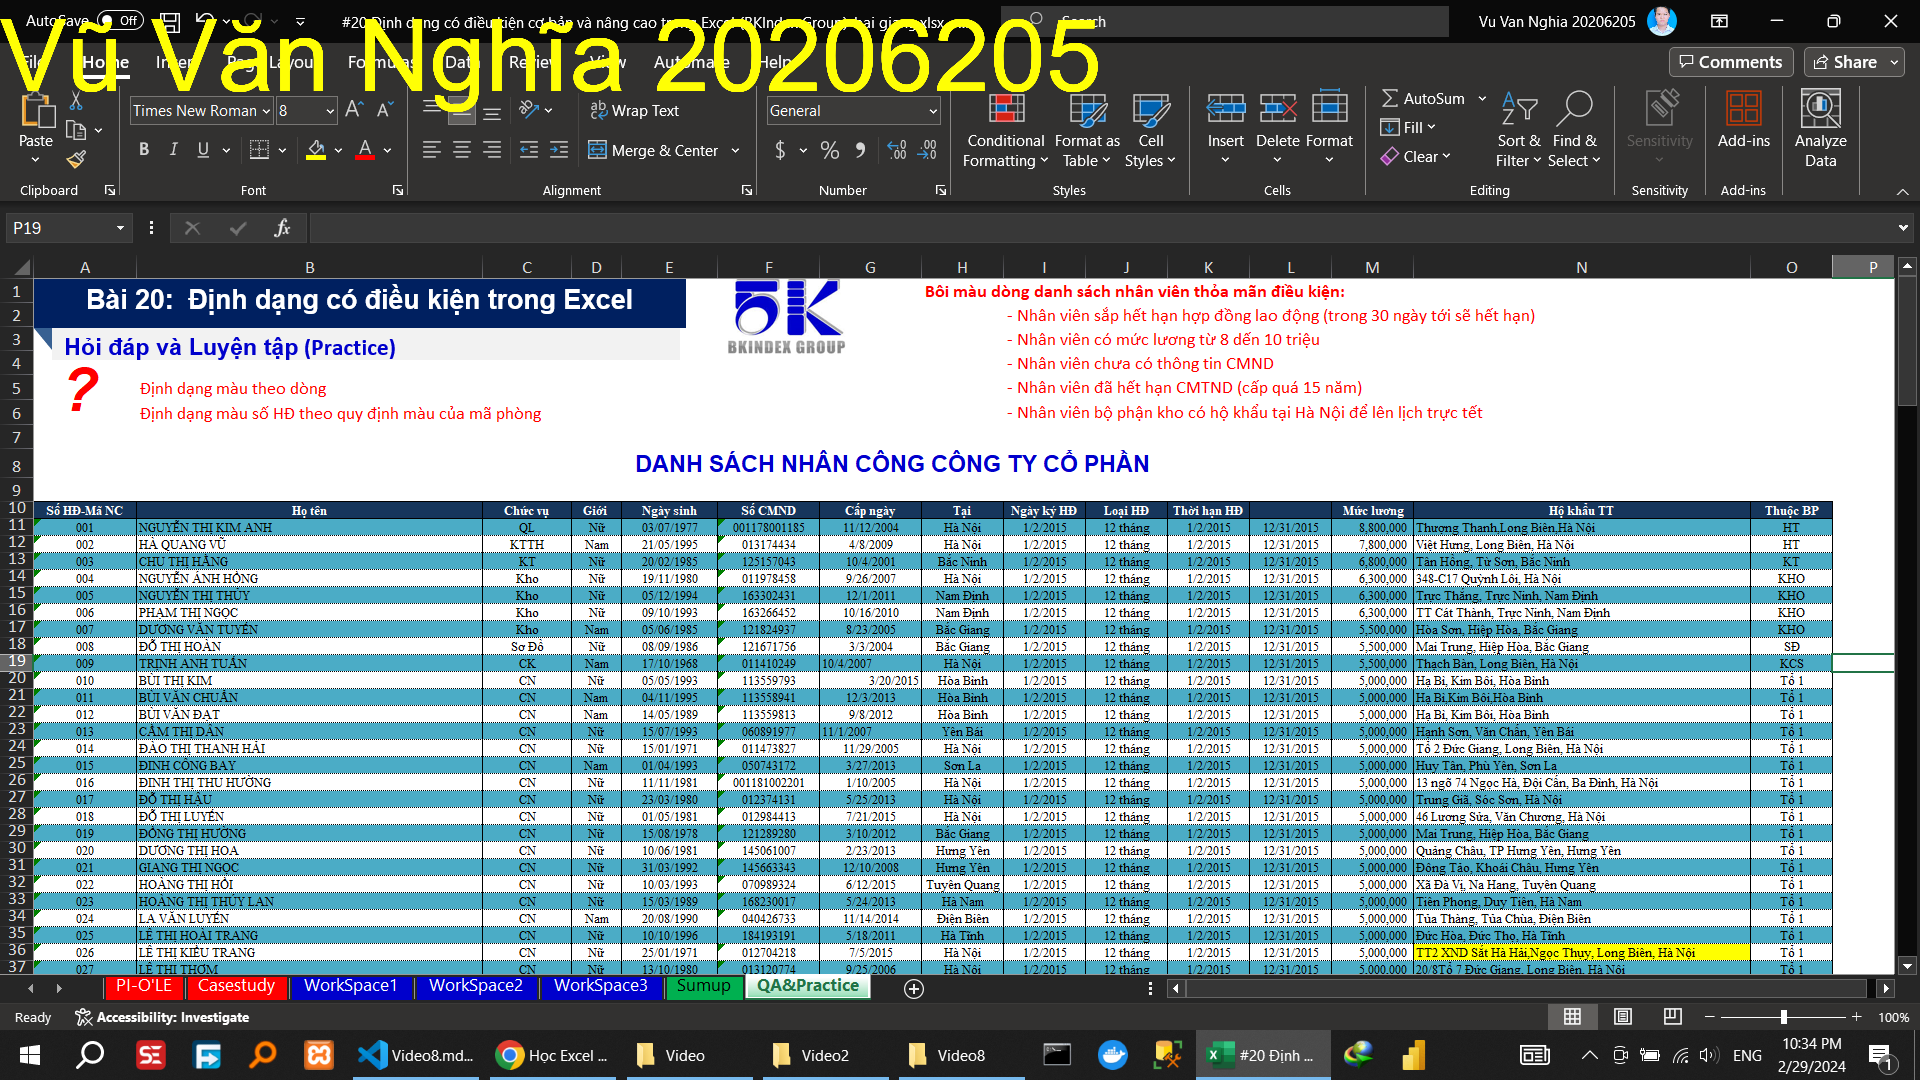
\includegraphics[scale = 0.15]{Video8/ThucHanh/0.png}
\caption{Thực hành định dạng màu theo dòng}
\end{figure}
\begin{figure}[h]
\centering
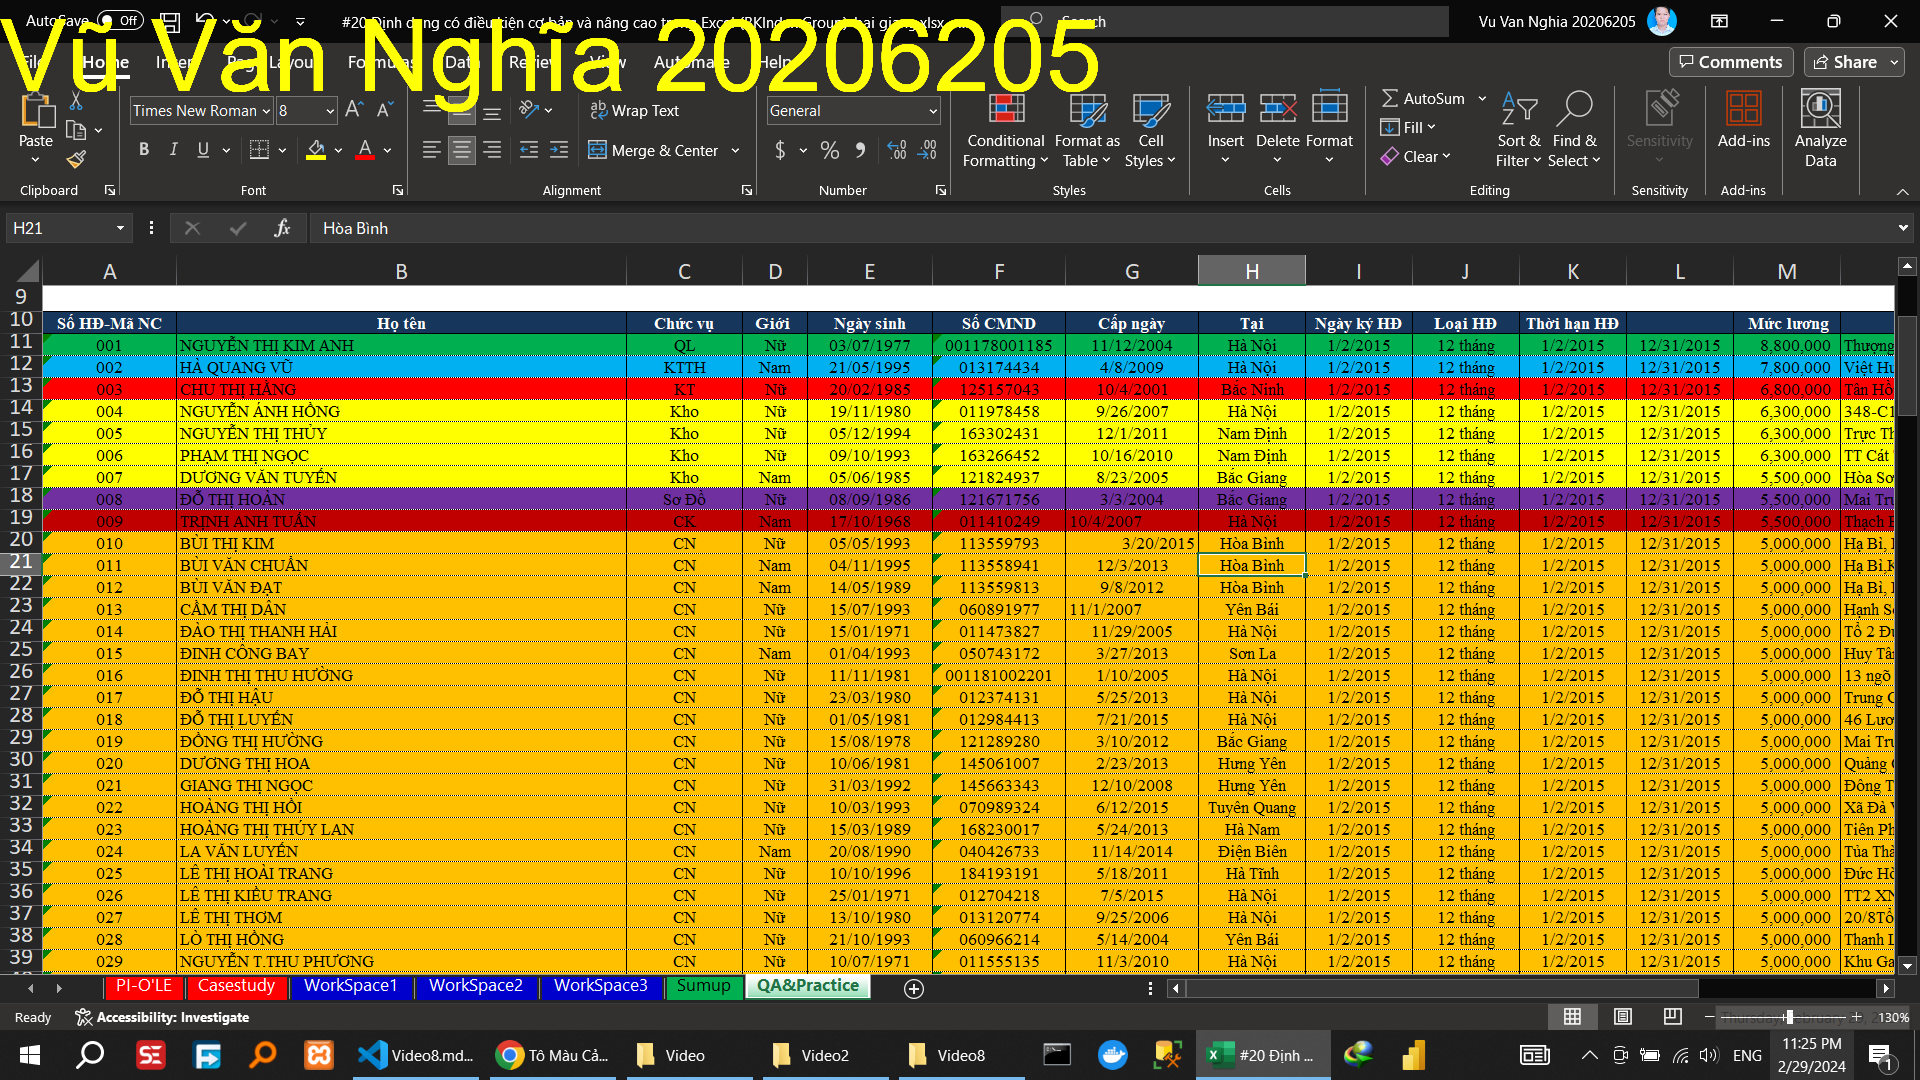
\includegraphics[scale = 0.15]{Video8/ThucHanh/1.png}
\caption{Thực hành định dạng màu số HĐ theo quy định màu của mã phòng}
\end{figure}
% =$L11-TODAY()<30
\begin{figure}[h]
\centering
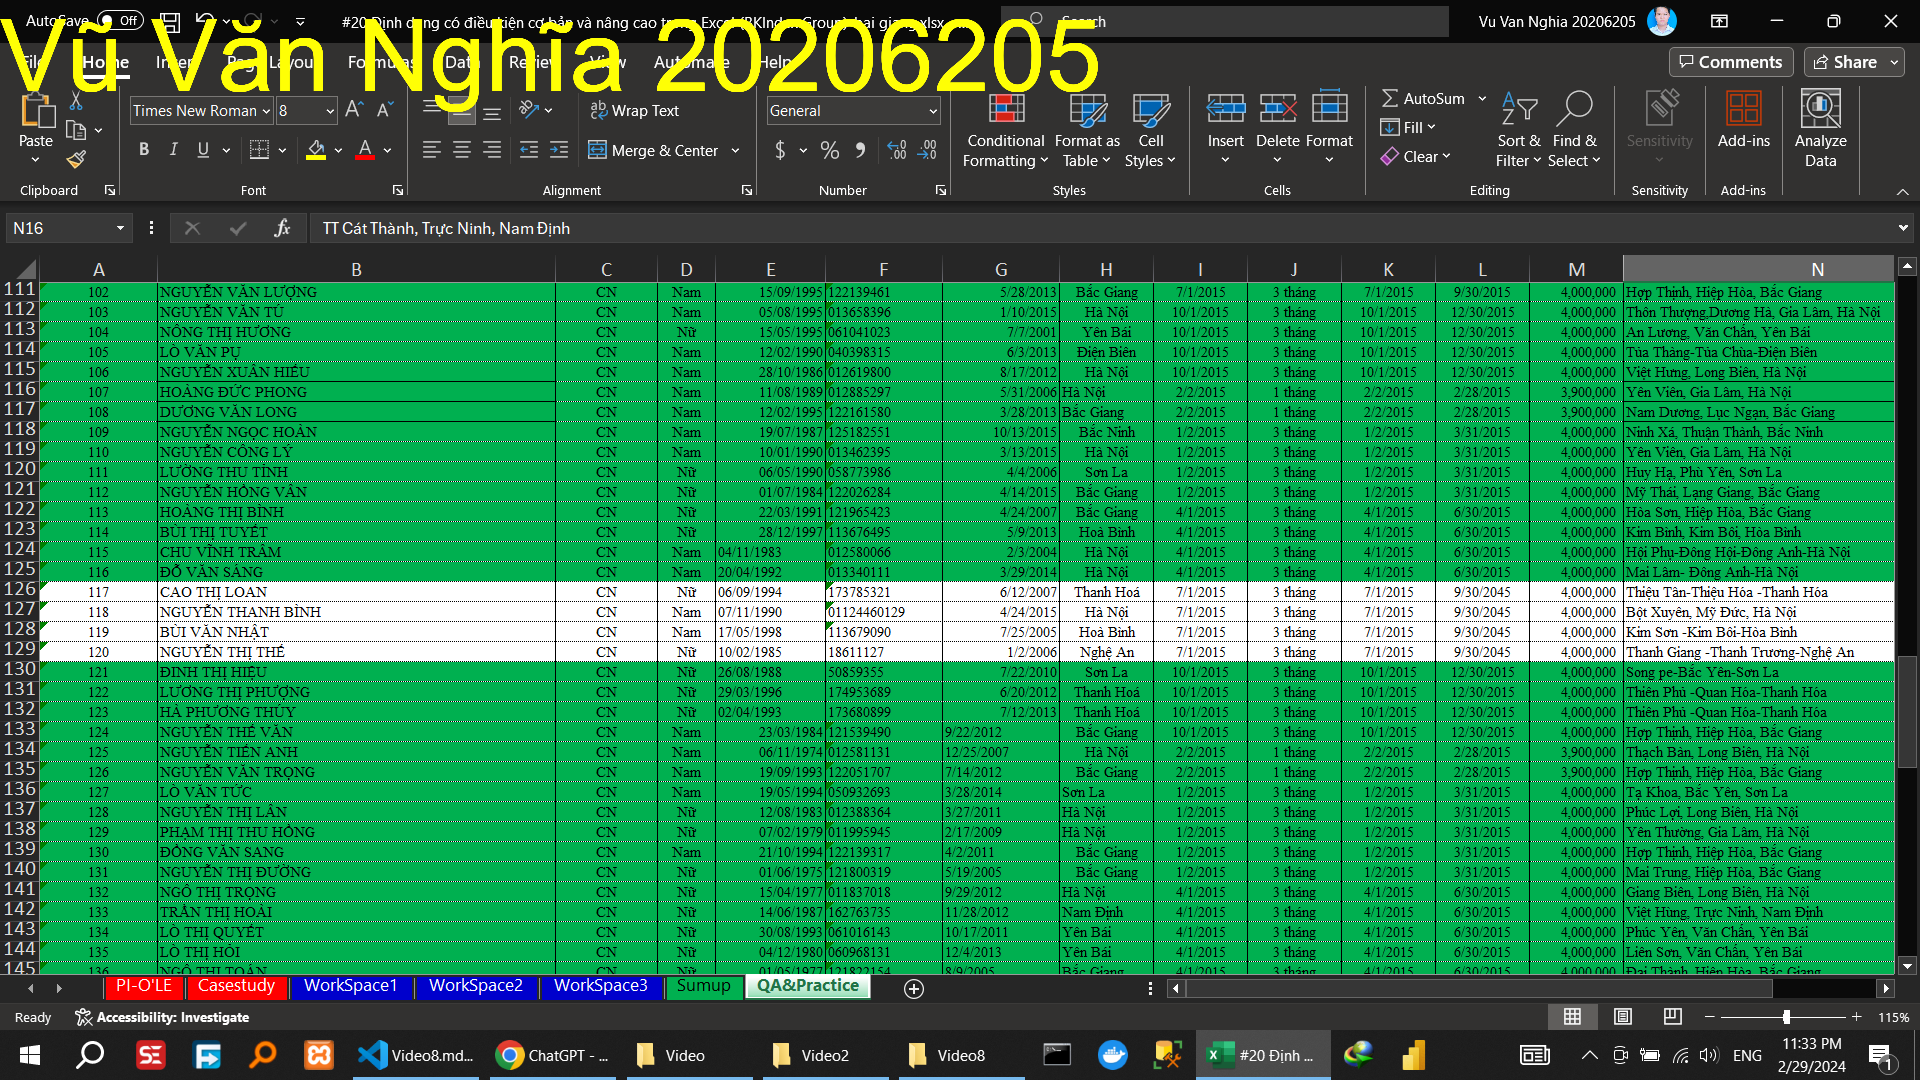
\includegraphics[scale = 0.15]{Video8/ThucHanh/2.png}
\caption{Thực hành định dạng màu: Nhân viên sắp hết hạn hợp đồng lao động (trong 30 ngày tới sẽ hết hạn)}
\end{figure}
% =AND($M11>=8000000, $M11<=10000000)
\begin{figure}[h]
\centering
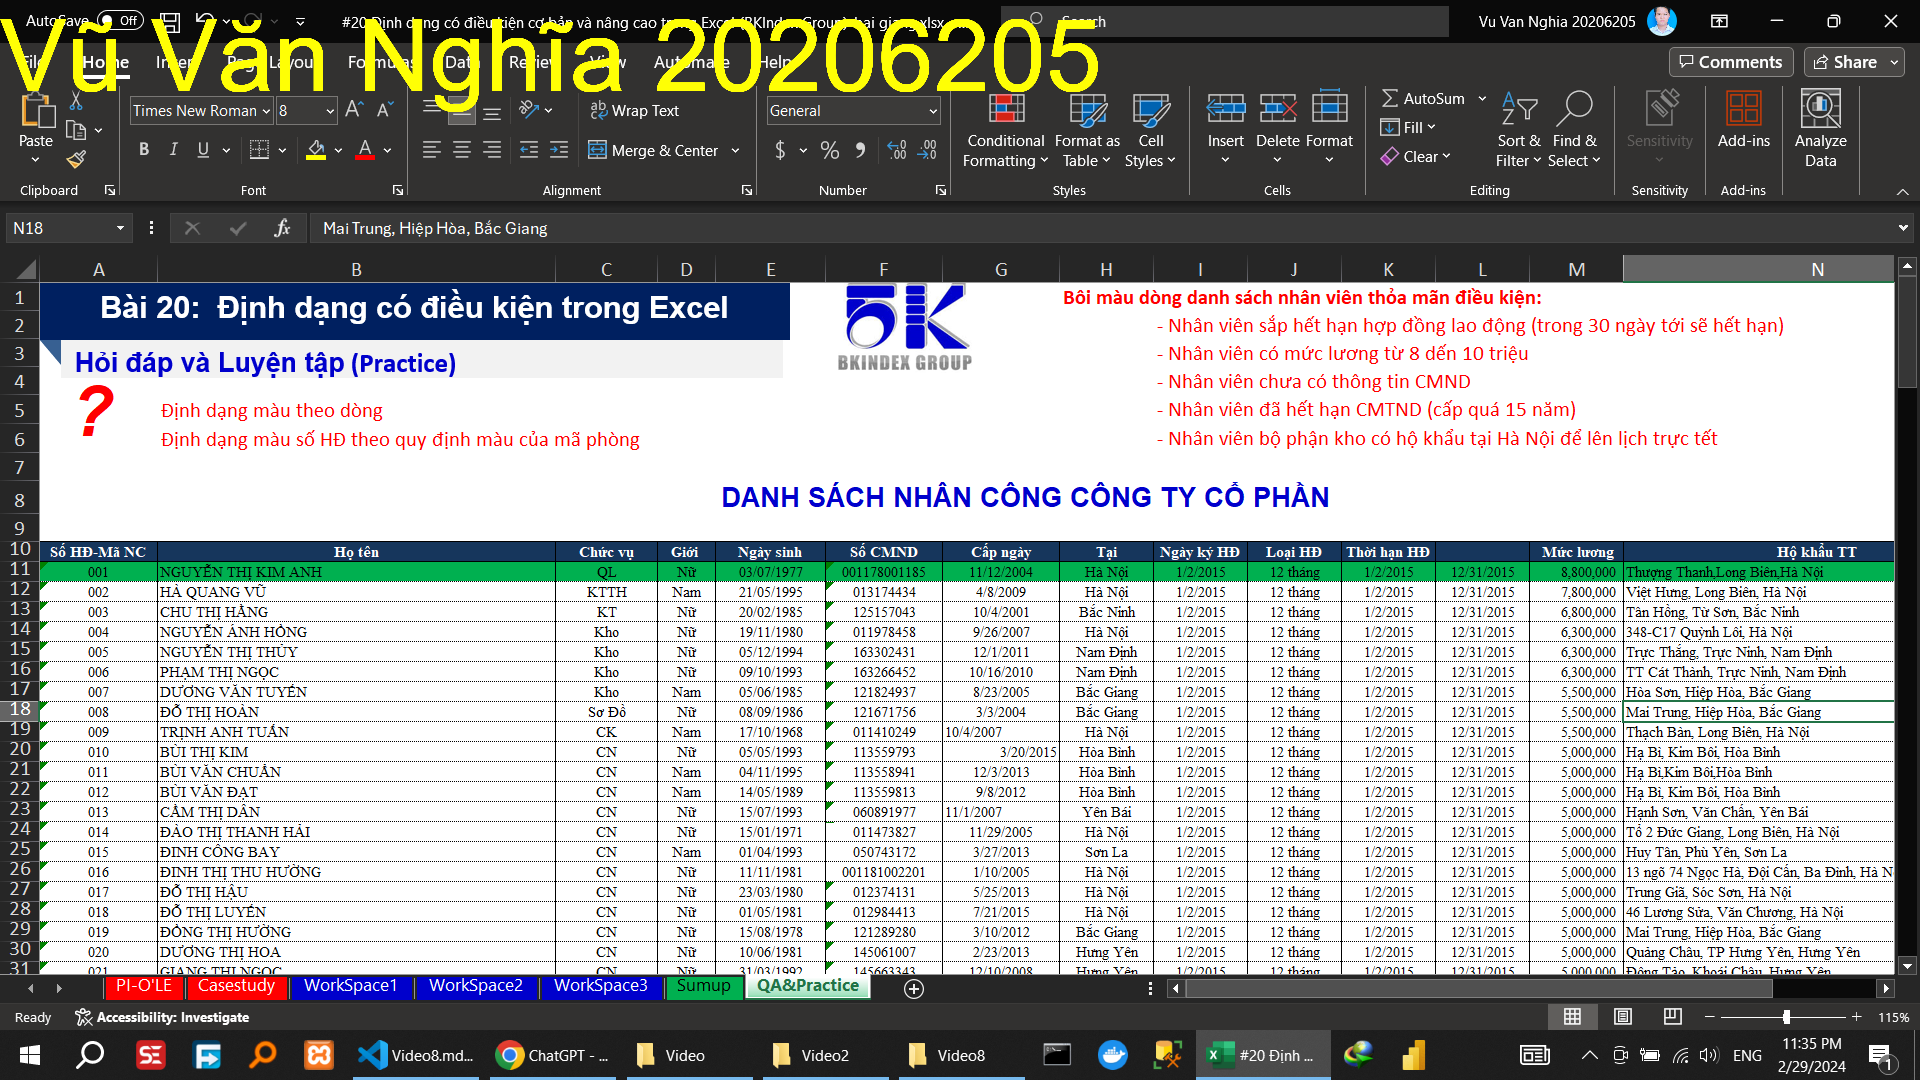
\includegraphics[scale = 0.15]{Video8/ThucHanh/3.png}
\caption{Thực hành định dạng màu: Nhân viên có mức lương từ 8 đến 10 triệu}
\end{figure}
% =$F11=""
\begin{figure}[h]
\centering
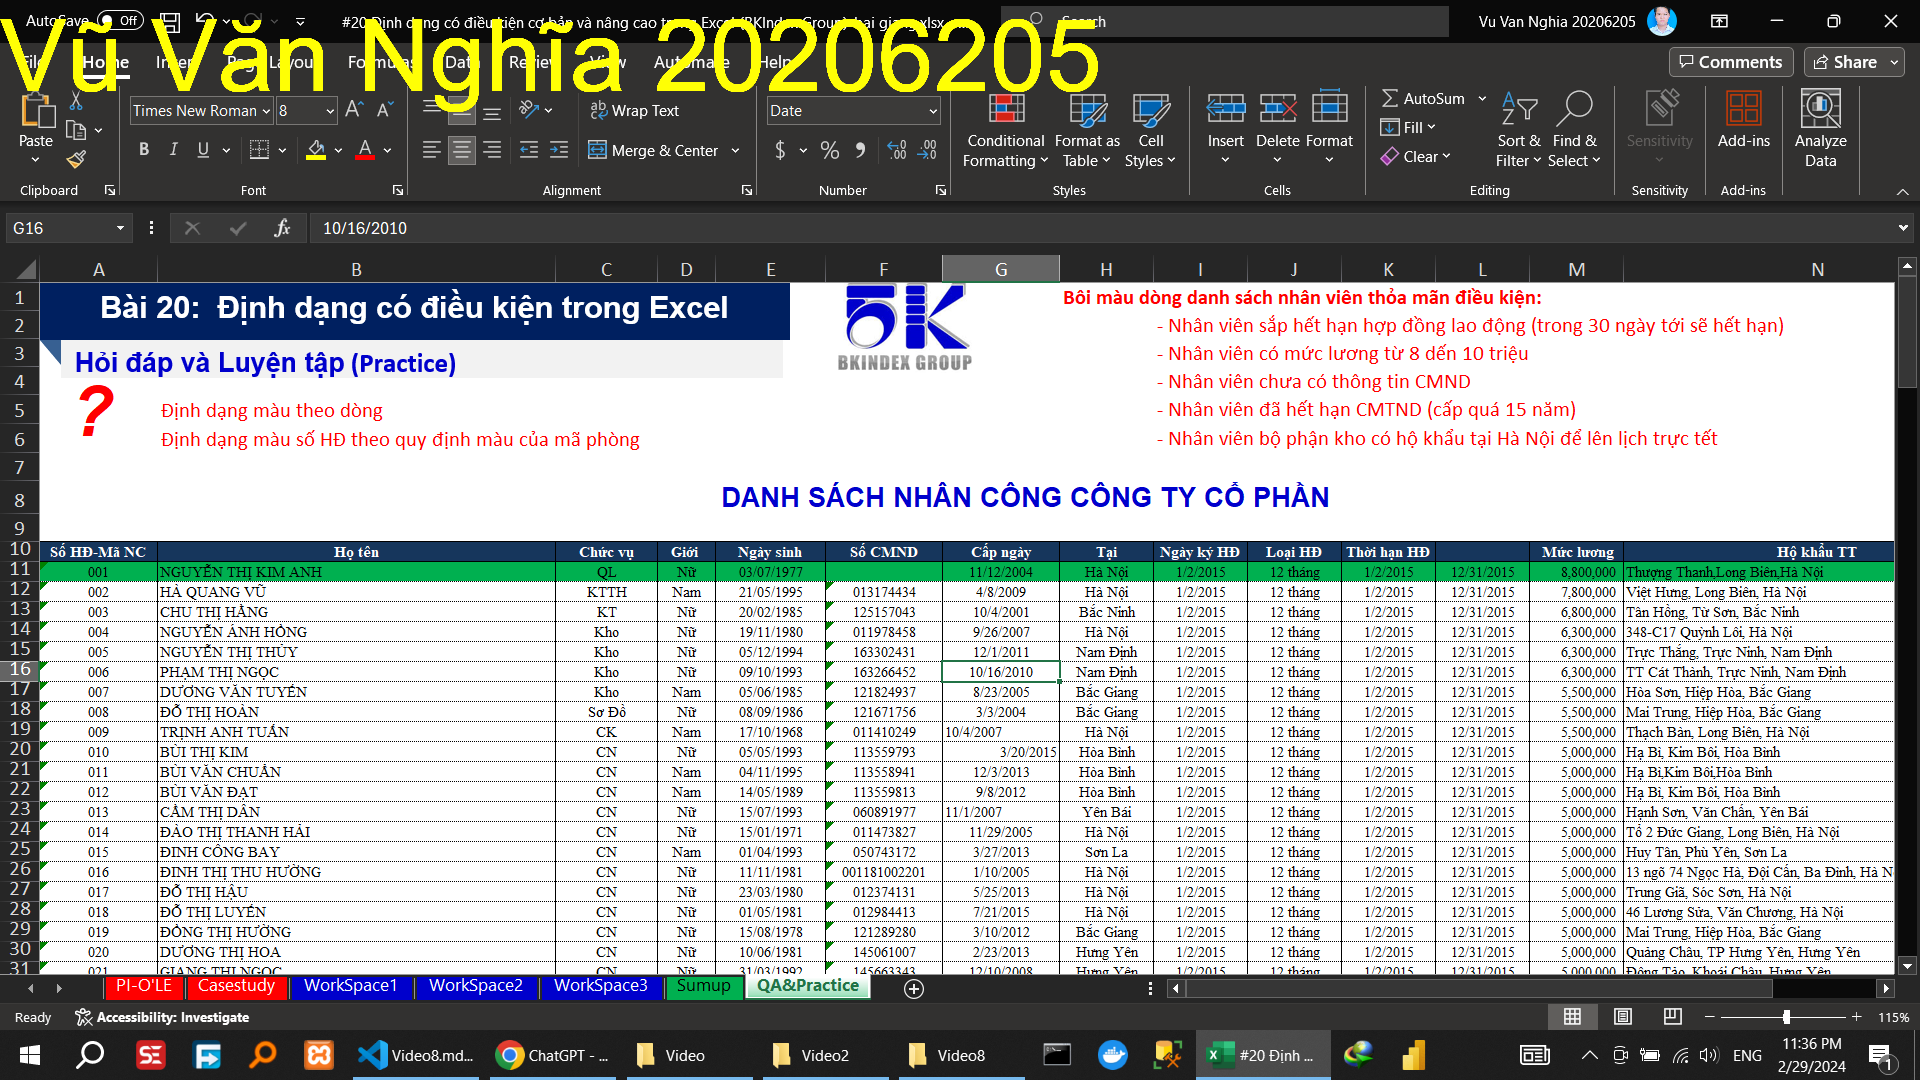
\includegraphics[scale = 0.15]{Video8/ThucHanh/4.png}
\caption{Thực hành định dạng màu: Nhân viên chưa có thông tin CMND}
\end{figure}
% =DATEDIF($G11, TODAY(), "y") > 15
\begin{figure}[h]
\centering
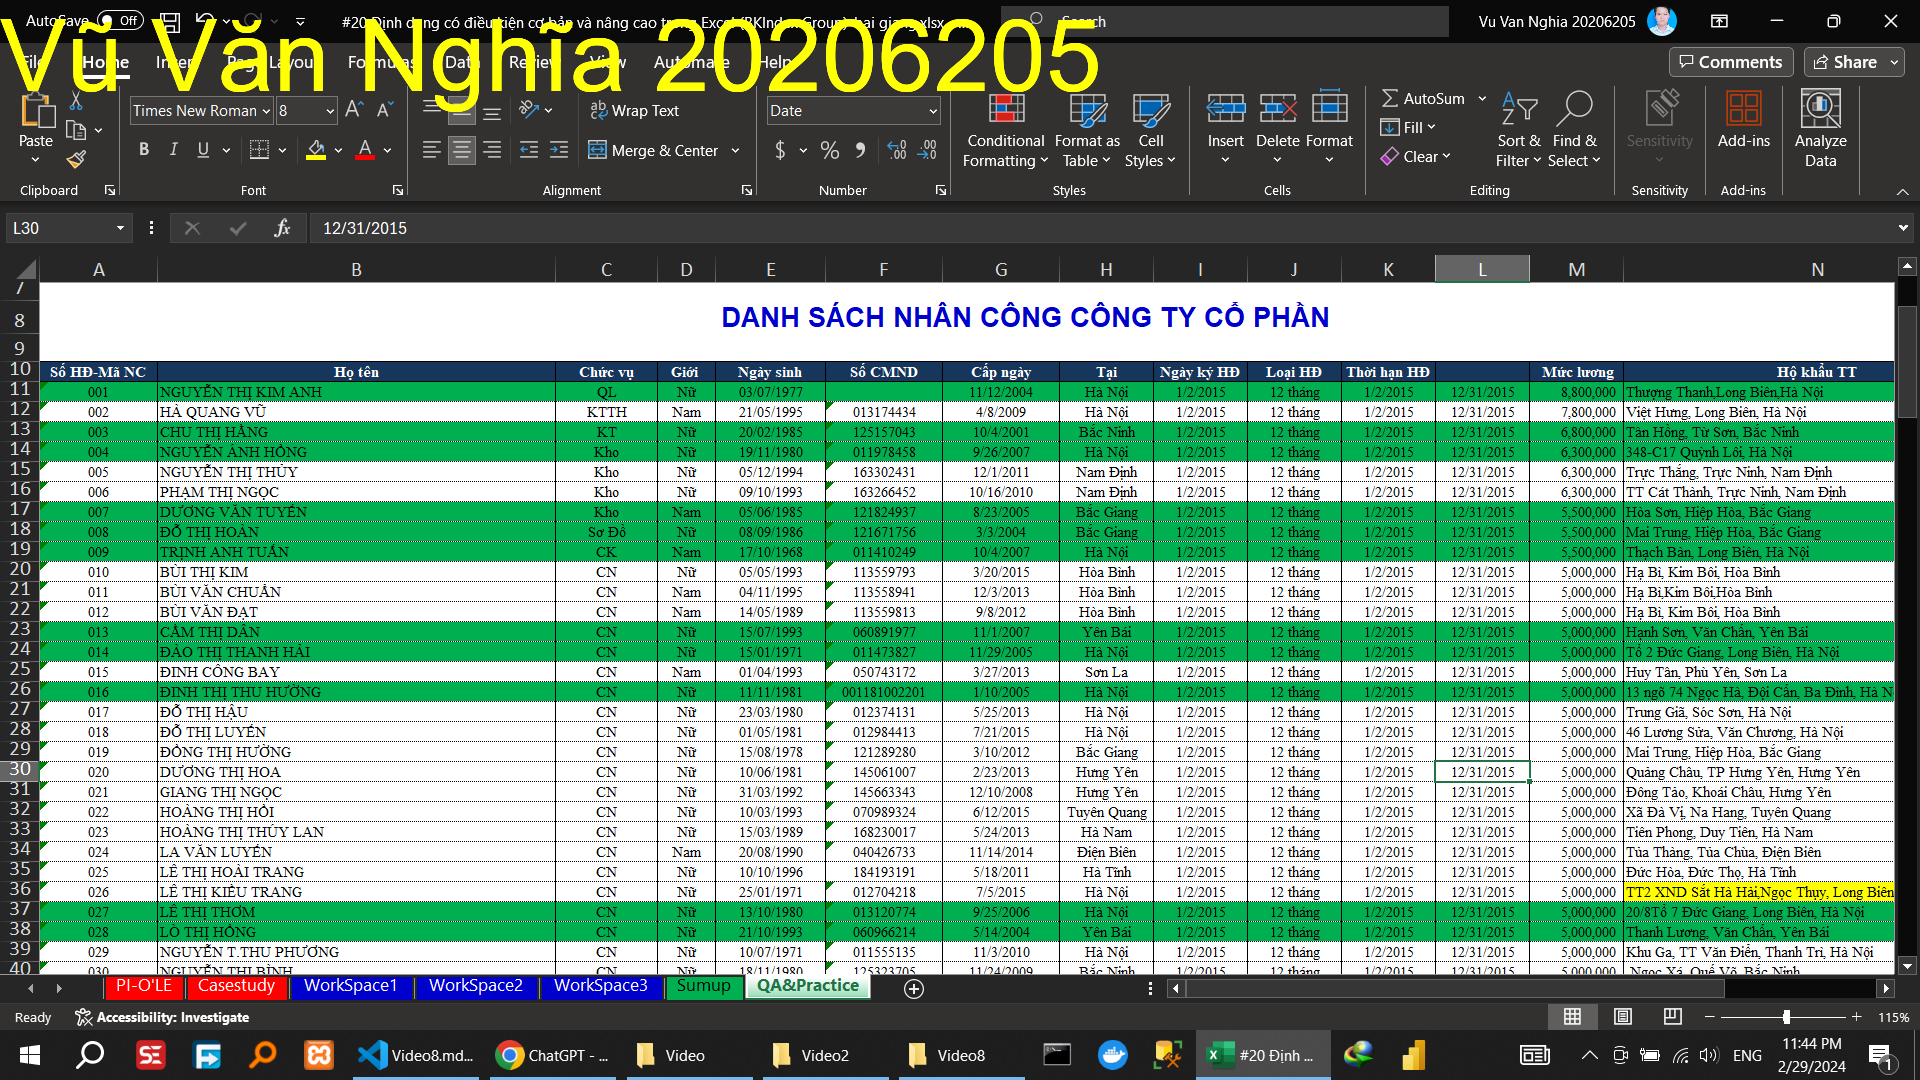
\includegraphics[scale = 0.15]{Video8/ThucHanh/5.png}
\caption{Thực hành định dạng màu: Nhân viên đã hết hạn CMTND (cấp quá 15 năm)}
\end{figure}
% =AND($C11="Kho", $H11="Hà Nội")
\begin{figure}[h]
\centering
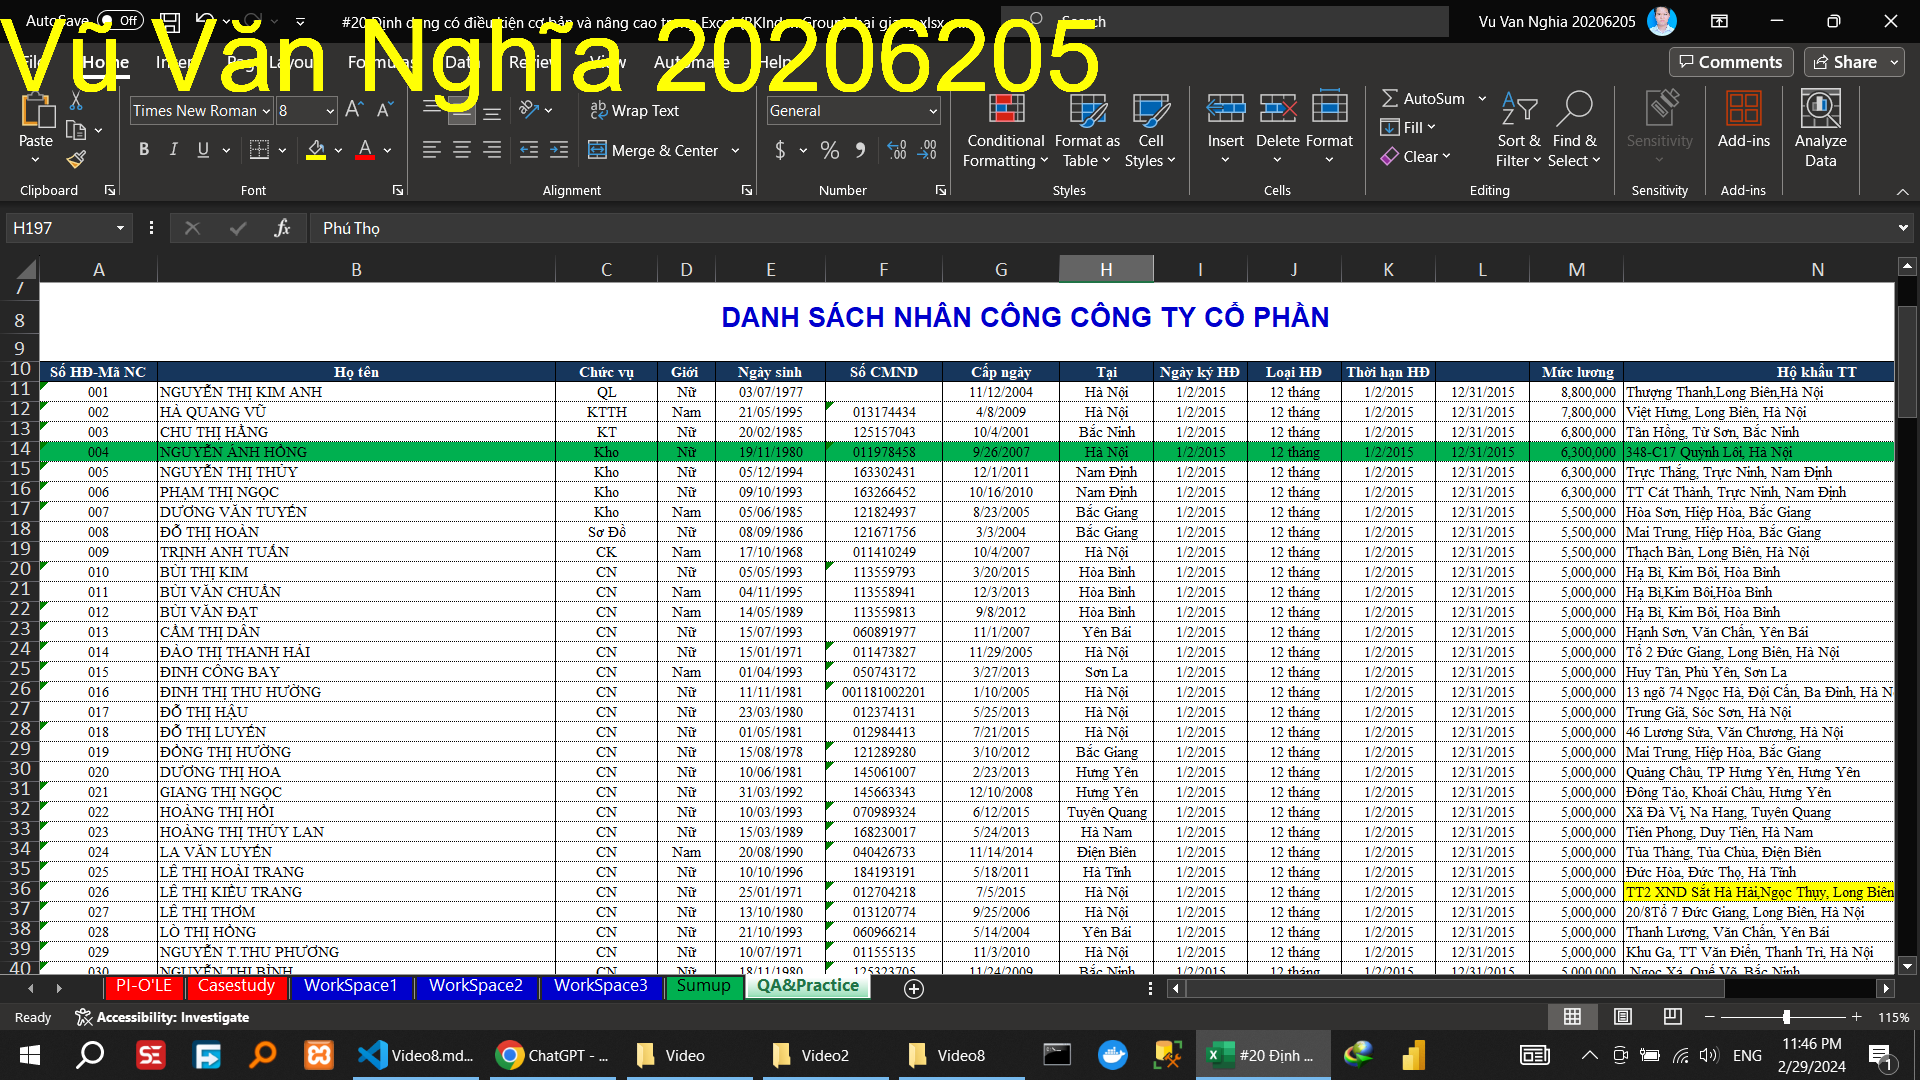
\includegraphics[scale = 0.15]{Video8/ThucHanh/6.png}
\caption{Thực hành định dạng màu: Nhân viên bộ phận kho có hộ khẩu tại HN để lên lịch trực tết}
\end{figure}
%%%%%%%%%%%%%%%%%%%%%%%%%%%%%%%%%%%%%%%%%%%%%%%%%%%%%%%
\end{document}
%%%%%%%%%%%%%%%%%%%%%%%%%%%%%%%%%%%%%%%%%%%%%%%%%%%%%%%